\chapter{バリデーション}
\section{実験概要}
\subsection{Video Cued-Recall メソッド}
インタラクティブ作品の評価方法にはさまざまな評価が存在するが、本作品を評価する上では、体験時、体験者がどのようなことに注意を向け、どのような行動を取ったかについて精緻に振り返る必要がある。そのため本研究では、体験者に体験時のようすをできるだけ詳細に表現してもらうため、Video Cued-Recallというメソッドを用いてデータの収集を行なった。 Video Cued-Recallとは、体験時のようすが記録された映像を視聴しながら、体験者本人が映像を手がかりに作品での体験を回顧し、言語化する方法である。インタビューを通して回顧するよりも詳細に体験を振り返ることができ、また体験しているそのときに体験のようすについて語ってもらう方法よりも、自然な体験について記述できることがその利点として挙げられる。

\subsection{参加者について}
インタビューは、FabCafe Nagoyaでの展示に際して、4名の体験者を対象に実施した。ただし、うち1名は「Relation」の体験時、トラッキングの精度が著しく低下していたため、1つ目に体験した「Familiar / Strange」の体験についてのみ調査の対象とした。

\subsection{データ収集}
参加者にはまず、調査の大まかな流れについて説明し、撮影についての許諾を得た。コンセプトの説明が自然な体験に影響することを避けるため、作品の体験の前にはコンセプトや具体的な作品の内容については説明せず、トラッキングされた手が次々に形を変えていくこと、手の形が表示された状態から始まり、再びもとの手の形に戻るループ構造のある作品であること、というインタビューに必要な最低限の構造のみ伝えた。

体験のようすは、手もとのハンドトラッキングを行うカメラ映像、現在時刻、体験者が実際に見ているスクリーンの映像が図\ref{fig:record_monitor}のようにレイアウトされて記録される。

\begin{figure}[H]
  \centering
  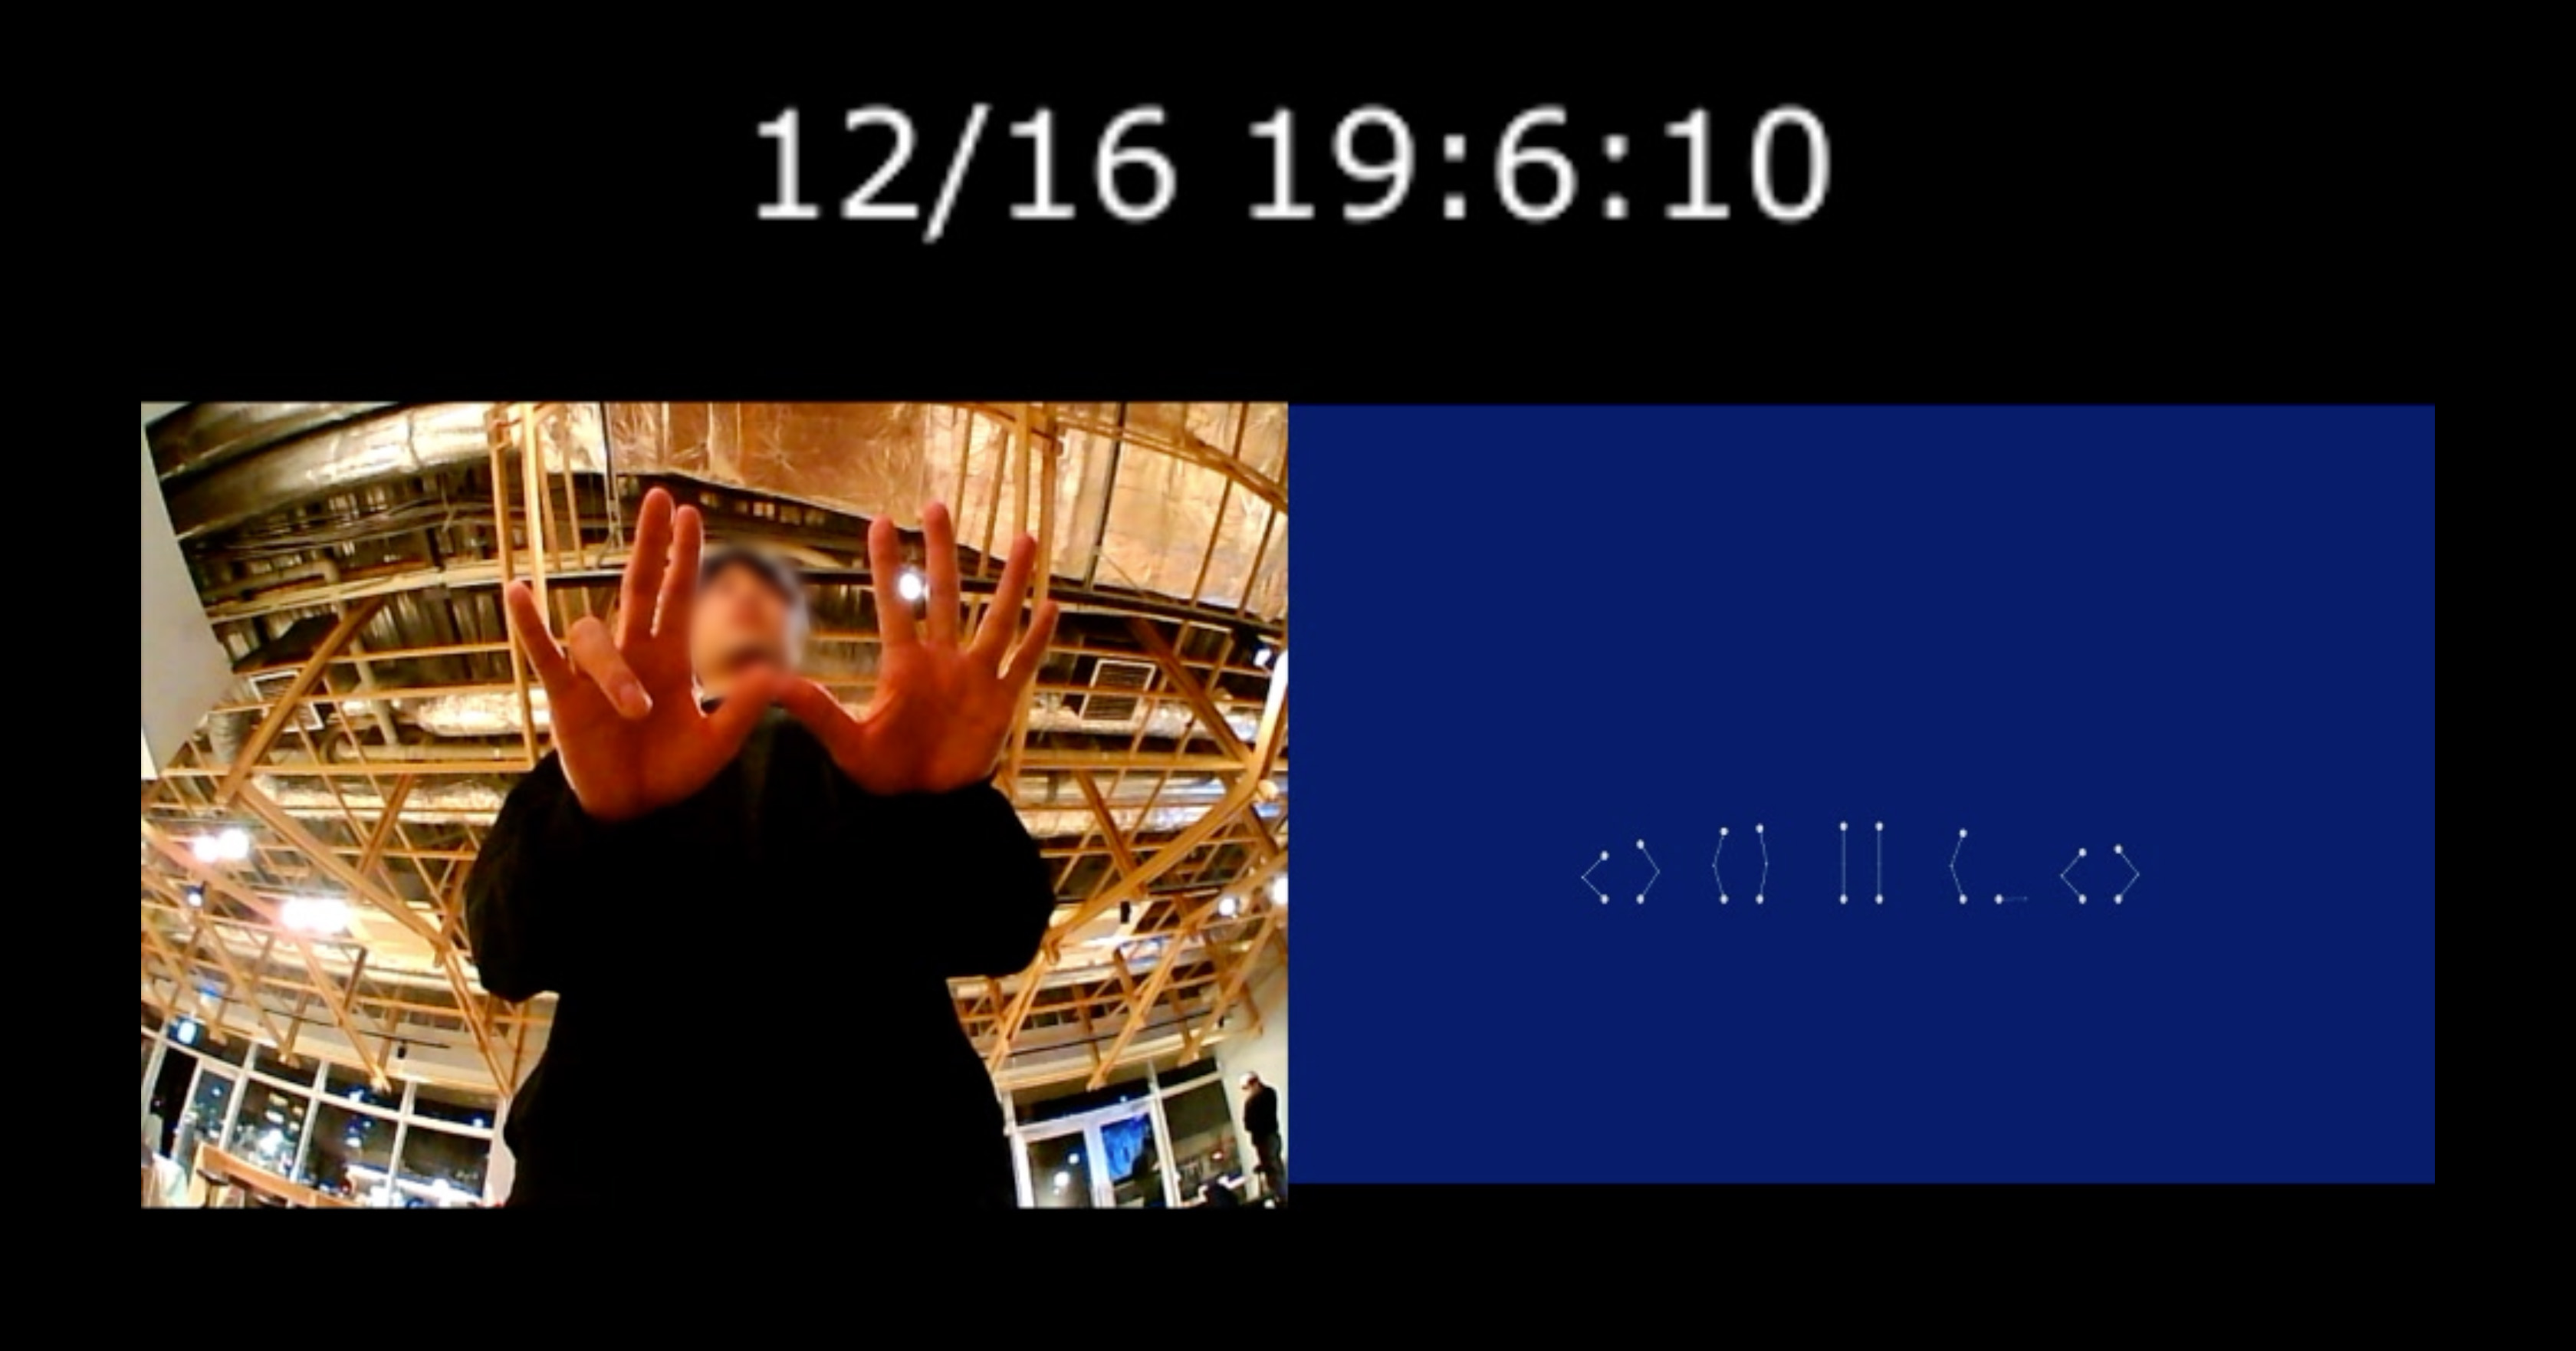
\includegraphics[width=15cm]{img/record_monitor.jpg}
  \caption{体験のようすの記録映像}
  \label{fig:record_monitor}
\end{figure}



\subsection{結果}
